% 图 5.10 (a) 反铁磁相（B 与 M+, M- 平行/反平行）(b) 自旋翻转跳跃相（M± 对称倾斜 theta=phi）
\documentclass[tikz,border=5pt]{standalone}
\usetikzlibrary{arrows.meta,calc}
\usepackage{amsmath}
\usepackage{bm}
\usepackage{fontspec}
\setmainfont{Times New Roman}
\begin{document}
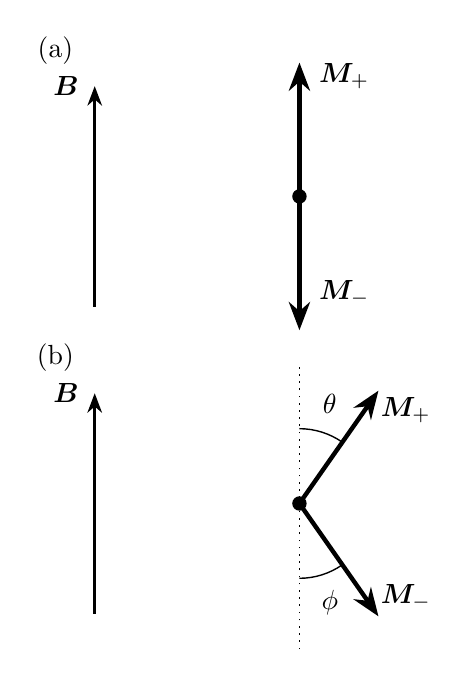
\begin{tikzpicture}[line width=0.8pt,>=Stealth]
% ---------- (a) ----------
\begin{scope}[shift={(0,0)}]
  \draw[->,line width=0.9] (-1.4,-0.1) -- (-1.4,2.7) node[left=2pt] {$\bm{B}$};
  \fill (1.2,1.3) circle (2.6pt);
  \draw[->,line width=1.6] (1.2,1.3) -- (1.2,3.0) node[right=3pt,pos=0.9] {$\bm{M}_+$};
  \draw[->,line width=1.6] (1.2,1.3) -- (1.2,-0.4) node[right=3pt,pos=0.72] {$\bm{M}_-$};
  \node at (-1.9,3.15) {(a)};
\end{scope}
% ---------- (b) ----------
\begin{scope}[shift={(0,-3.9)}]
  \draw[->,line width=0.9] (-1.4,-0.1) -- (-1.4,2.7) node[left=2pt] {$\bm{B}$};
  \fill (1.2,1.3) circle (2.6pt);
  \draw[dotted,line width=0.6] (1.2,-0.55) -- (1.2,3.05);
  \draw[->,line width=1.6] (1.2,1.3) -- ++(55:1.75);
  \node[right=2pt] at ($(1.2,1.3)+(55:1.45)$) {$\bm{M}_+$};
  \draw[->,line width=1.6] (1.2,1.3) -- ++(-55:1.75);
  \node[right=2pt] at ($(1.2,1.3)+(-55:1.45)$) {$\bm{M}_-$};
  \draw[line width=0.5] ($(1.2,1.3)+(90:0.95)$) arc[start angle=90,end angle=55,radius=0.95];
  \node at ($(1.2,1.3)+(73:1.32)$) {$\theta$};
  \draw[line width=0.5] ($(1.2,1.3)+(-90:0.95)$) arc[start angle=-90,end angle=-55,radius=0.95];
  \node at ($(1.2,1.3)+(-73:1.32)$) {$\phi$};
  \node at (-1.9,3.15) {(b)};
\end{scope}
\end{tikzpicture}
\end{document}
